% !TeX TXS-program:compile = txs:///pdflatex/[--shell-escape]

\documentclass[9pt]{beamer}
\usetheme{Madrid}
\usecolortheme{beaver}
\usepackage{amsmath,amssymb,amsthm,asymptote,graphicx}
\usepackage{graphics}
% \usepackage{bisvslides}
\usepackage{arcs}
\graphicspath{{./images}}

\newcounter{problem}[section]

\newenvironment{probslide}[3][]{%
    \refstepcounter{problem}\begin{frame}[t]%
	{Problem \thesection.\theproblem 
        \def\temp{#2}\ifx\temp\empty
            %
        \else
            \ - \temp%
        \fi}
    {#3}}%
	{\end{frame}}

% \newenvironment{Example}[2][Example]
%     {This is an #1. You gave #2 as an argument. The rest will be bold: \bfseries}
%     {}
% \textbf{Problem~\theproblem. #1
% \newenvironment{bsmi}{\begin{CJK}{UTF8}{bsmi}}{\end{CJK}}

\title{Geometry}
\subtitle{Mathcounts 21 - Session 3}
\author{Rohan D., Derrick L.}
\institute{BISV Mathcounts Club 21}
\date{December 7, 2021}

%\maketitle
%~~~~~~~~~~~~~~~~~~~~~~~~~~~~~~~~~~~~~~~~~~~~~~~~~~~~~~~~~~~~~~~~~~~~~~~~~~~~~~
% Informations
%\title{TEMPLATE}

%\titlegraphic{assets/gkg.png} %change this to your preferred logo or image(the image is located on the top right corner).
%~~~~~~~~~~~~~~~~~~~~~~~~~~~~~~~~~~~~~~~~~~~~~~~~~~~~~~~~~~~~~~~~~~~~~~~~~~~~~~

\begin{document}

% Generate title page
\begin{frame}
    \titlepage        
\end{frame}
% \setbeamertemplate{footline}[miniframes Madrid]

\setcounter{section}{7}
\section{Beginner Practice Problems}


\begin{frame}[t, fragile]{Problem \thesection.\theproblem}
    \begin{block}{}
    The surface area of a cube is 294 square inches. What is the number of inches in the length of one of the
edges?
	TBD D
    \end{block}
\end{frame}
% \end{document}

\refstepcounter{problem}
\begin{frame}[t, fragile]{Problem \thesection.\theproblem}
    \begin{block}{}[Mathcounts 2017 Chapter, Target \#1]
     What is the area, in square units, of the rectangle with vertices $A(0, 0), B(0, 3), C(2, 3)$ and $D(2, 0)?$
     
    \end{block}
\end{frame}

\refstepcounter{problem}
\begin{frame}[t, fragile]{Problem \thesection.\theproblem}
    \begin{block}{}[Mathcounts]
    %  Concept: Geometry • Difficulty: 3 • Answer: 0.51 • Solution Available: Yes (Hide) • Report an error with this problem.

 The diagram shows eight congruent squares inside a circle. Every shaded square has one vertex on the circle. What is the ratio of the shaded area to the area of the circle? Express your answer as a decimal to the nearest hundredth.

    \end{block}
    \begin{center}
        \begin{asy}
        import cse5;
    size(100);
    filldraw((0,0)--(2,0)--(2,1)--(0,1)--cycle,mediumgrey);
    draw((1,0)--(1,1));
    filldraw((0,3)--(2,3)--(2,4)--(0,4)--cycle,mediumgrey);
    draw((1,3)--(1,4));
    filldraw((2,1)--(3,1)--(3,3)--(2,3)--cycle,mediumgrey);
    draw((2,2)--(3,2));
    filldraw((-1,1)--(0,1)--(0,3)--(-1,3)--cycle,mediumgrey);
    draw((-1,2)--(0,2));
    draw(Circle((1,2),sqrt(5)));
            
        \end{asy}
    \end{center}
    
    \end{frame}


\refstepcounter{problem}
\begin{frame}[t, fragile]{Problem \thesection.\theproblem}
    \begin{block}{}[Mathcounts]
      How many congruent 4-foot tall cylindrical pipes with an inside diameter of 2 inches are needed to hold the same amount of water as one pipe of the same height with an inside diameter of 12 inches?
      
      
    \end{block}
\end{frame}

\refstepcounter{problem}
\begin{frame}[t, fragile]{Problem \thesection.\theproblem}
    \begin{block}{}[Mathcounts]
    A can is in the shape of a right circular cylinder. The circumference of the base of the can is 12 inches, and the height of the can is 5 inches. A spiral strip is painted on the can in such a way that it winds around the can exactly once as it reaches from the bottom of the can to the top. It reaches the top of the can directly above the spot where it left the bottom. What is the length in inches of the stripe?

     
    \end{block}
    \begin{center}
        \begin{asy}
            import cse5;
            size(120);
            draw(shift(1.38,0)*yscale(0.3)*Circle((0,0), .38));
            
            draw((1,0)--(1,-2));
            draw((1.76,0)--(1.76,-2));
            
            draw((1,-2)..(1.38,-2.114)..(1.76,-2));
            path p =(1.38,-2.114)..(1.74,-1.5)..(1,-0.5)..(1.38,-.114);
            pair a=(1.38,-2.114), b=(1.76,-1.5);
            path q =subpath(p, 1, 2);
            path r=subpath(p,0,1);
            path s=subpath(p,2,3);
            draw(r);
            draw(s);
            draw(q, dashed);
            
            label("$5$",midpoint((1.76,0)--(1.76,-2)),E);
            
        \end{asy}
    \end{center}


\end{frame}

\refstepcounter{problem}
\begin{frame}[t, fragile]{Problem \thesection.\theproblem}
    \begin{block}{}[Mathcounts]
    %  Concept: Geometry • Difficulty: 3 • Answer: $972\pi$ cubic cm • Solution Available: Yes (Hide) • Report an error with this problem.

 The surface area of a particular sphere is $324\pi\text{ cm}^2$. What is the volume, in cubic centimeters, of the sphere? Express your answer in terms of $\pi$.
    
    \end{block}
\end{frame}

\refstepcounter{problem}
\begin{frame}[t, fragile]{Problem \thesection.\theproblem}
    \begin{block}{}[Mathcounts]
    %  Concept: Geometry • Difficulty: 3 • Answer: 4.1 cm • Solution Available: Yes (Hide) • Report an error with this problem.

 Circle $P$ has radius 10 cm. Two perpendicular radii are drawn, and a smaller circle is drawn tangent to both radii and the larger circle, as shown. What is the radius of the smaller circle? Express your answer as a decimal to the nearest tenth.

    
    \end{block}
    \begin{center}
        \begin{asy}
        import cse5;
        size(150);
        draw(Circle((0,0),10));
        dot((0,0));
        label("$P$",(0,0),SW);
        draw((0,0)--(10,0));
        draw((0,0)--(0,10));
        real r=10*sqrt(2)-10;
        draw(Circle((r,r),r));
            
        \end{asy}
    \end{center}
 
\end{frame}
%------------------------------------------------------

\section{Intermediate Practice Problems}

\refstepcounter{problem}
\begin{frame}[t, fragile]{Problem \thesection.\theproblem}
    \begin{block}{}[Purple Comet 2018, \#10]
    The triangle below is divided into nine stripes of equal width each parallel to the base of the triangle. The darkened stripes have a total area of $135.$ Find the total area of the light colored stripes.
     
    \end{block}
    \begin{center}
        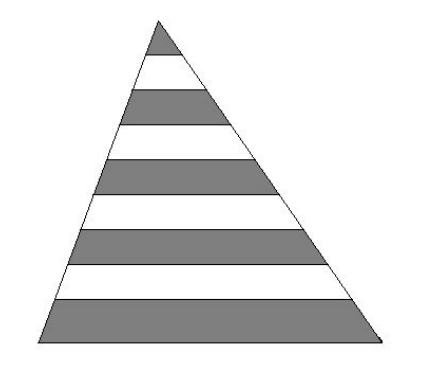
\includegraphics[]{pc_2018_10}
    \end{center}
    
\end{frame}
\refstepcounter{problem}
\begin{frame}[t, fragile]{Problem \thesection.\theproblem}
    \begin{block}{}[Mathcounts 2017 Chapter, Sprint \#2]
     A circle is inscribed in a right isosceles triangle whose legs are 8 inches long.
    How many square inches are in the area of the shaded portion? Express your answer as a decimal rounded to the nearest hundredth.
    
    \end{block}
    \begin{center}
        \begin{asy}
            unitsize (0.5cm);
            real x = 4*sqrt(2);
            real r = 8 - x;
            pair A = (0, r*sqrt(2));
            pair B = (-x, -r);
            pair C = (x, -r);
            
            filldraw (A--B--C--cycle, gray(0.85), black);
            filldraw (circle ((0,0), r), white, black);
        \end{asy}
    \end{center}
\end{frame}
\refstepcounter{problem}
\begin{frame}[t, fragile]{Problem \thesection.\theproblem}
    \begin{block}{}[Mathcounts]
     In square $ABCD$, shown here, sector $BCD$ was drawn with a center $C$ and $BC = 24 \text{ cm}$. A semicircle with diameter $AE$ is drawn tangent to the sector $BCD$. If points $A$, $E$ and $D$ are collinear, what is $AE$?


    
    \end{block}
    \begin{center}
        \begin{asy}
            import cse5;
            pair A,B,C,D,E,F;
            unitsize(4cm);
            D = (0,-1); C = (1,-1); B = (1,0); E = (0, -0.5); F = (0, -0.25);
            draw(arc(C,1,90,180));
            draw(arc(F,0.25,-90,90));
            draw(B--A--D--C--B);
            label("$A$",A,W); label("$B$",B,N); label("$C$",C,E); label("$D$",D,W); label("$E$",E,W);
                    
        \end{asy}
        \end{center}
    
    \end{frame}

\refstepcounter{problem}
\begin{frame}[t, fragile]{Problem \thesection.\theproblem}
    \begin{block}{}[Mathcounts 2017, Chapter \#28]
     In right triangle $ABC,$ shown here, $m\angle{B} = 90^\circ$ and $AB = 6$ inches. If inscribed circle $Q$ has area $4\pi \text{ in}^2,$ what is the area of triangle $ABC?$
    \end{block}
    \begin{center}
        \begin{asy}
            unitsize (0.5cm);
            pair B = (0, 0);
            pair A = (0, 6);
            pair C = (8, 0);
            pair Q = (2, 2);
            
            draw (A--B--C--cycle);
            draw (circle (Q, 2));
            
            label ("$A$", A, N);
            label ("$B$", B, SW);
            label ("$C$", C, SE);
            dot ("$Q$", Q, SE);
        \end{asy}
    \end{center}
    
\end{frame}

% \emph{Difficulty:} 5 (Mathcounts)
\refstepcounter{problem}
\begin{frame}[t, fragile]{Problem \thesection.\theproblem}
    \begin{block}{}[Mathcounts]
Two semicircles are inscribed in a rectangle as shown so their diameters are opposite sides of the rectangle. What is the probability that a point randomly selected inside the rectangle will also be inside both semicircles? Express your answer as a decimal rounded to the nearest hundredth. (You may use calculator for this.)

    \end{block}
    \begin{center}
        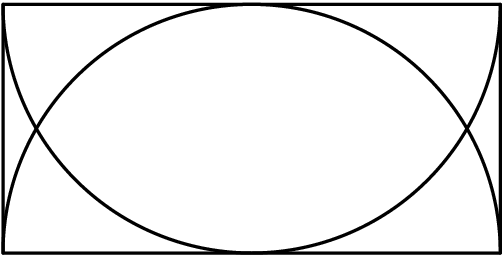
\includegraphics[scale=0.5]{images/38bfd76b3eb6bc5f6291aca8255bd167b545e722.png}
        \end{center}
        
        \end{frame}
% \begin{answer*}
% 0.61
% \end{answer*}

\refstepcounter{problem}
\begin{frame}[t, fragile]{Problem \thesection.\theproblem}
    \begin{block}{}[Mathcounts]
    %  Concept: Geometry • Difficulty: 5 • Answer: 12 units • Solution Available: Yes (Hide) • Report an error with this problem.

 In circle $O$, shown, $OP=2\text{ units}$, $PL=8\text{ units}$, $PK=9\text{ units}$ and $NK=18\text{ units}$. Points $K, P,$ and $M$ are collinear, as are points $L, P, O,$ and $N.$ What is the length of segment $MN$?

    \end{block}
    \begin{center}
        \begin{asy}
            unitsize(0.33cm);
            draw(circle((0,0),10),black+linewidth(1));
            draw((0,10)--(0,-10)--(9.5,3.12)--(0,10)--(-7,-7.14)--(9.5,3.12),black+linewidth(1));
            dot((0,0));
            label("$N$",(0,10),N);
            label("$L$",(0,-10),S);
            label("$M$",(9.5,3.12),E);
            label("$K$",(-7,-7.14),SW);
            label("$P$",(0,-2.5),SE);
            label("$O$",(0,0),W);
            
        \end{asy}
    \end{center}
        
    \end{frame}
%2012 State Sprint Round, 17
\refstepcounter{problem}
\begin{frame}[t, fragile]{Problem \thesection.\theproblem}
    \begin{block}{}[Mathcounts 2012 State Sprint Round, \#23]
    In trapezoid $ABCD$ segments $AB$ and $CD$ are parallel. Point $P$ is the intersection of diagonals $AC$ and $BD$. The area of $\triangle{PAB}$ is 16 square units, and the area of $\triangle{PCD}$ is 25 square units. What is the area of trapezoid $ABCD$?
    \end{block}
    \begin{center}
        \begin{asy}
        import cse5;
        
        unitsize (0.6cm);
        
        pair A, B, C, D, P, X, Y;
        D = (0,0);
        A = (2,3);
        B = (6,3);
        C = (8,0);
        
        P = intersectionpoint(A--C, B--D);
        
        draw(A--B--C--D--cycle);
        draw(A--C);
        draw(B--D);
        
        label("$A$", A, N);
        label("$B$", B, N);
        label("$C$", C, S);
        label("$D$", D, S);
        label("$P$", P, S);
        
        \end{asy}
        
    \end{center}     
    
\end{frame}




%259, 12-13, Plane Geometry 7
\refstepcounter{problem}
\begin{frame}[t, fragile]{Problem \thesection.\theproblem}
    \begin{block}{}[Mathcounts  2012-13 Handbook, \#259]
    In rectangle $ABCD$, point $E$ lies on $\overline{BC}$ so that $\cfrac{BE}{BC} = 2$ and point $F$ lies on $\overline{DC}$ so that $\cfrac{CF}{FD} = 2$. Segments $AE$ and $AC$ intersect $BF$ at points $X$ and $Y$, respectively. The extended ratio $FY:YX:XB = a:b:c$ so that $a, b$ and $c$ are relatively prime positive integers. What is the value of $a + b + c$? 

    \end{block}
    \begin{center}
        \begin{asy}
        import cse5;
        
        unitsize (0.75cm);
        
        pair A, B, C, D, E, F, X, Y;
        D = (0,0);
        A = (0,3);
        B = (6,3);
        C = (6,0);
        F = (2, 0);
        E = (6, 1);
        
        X = intersectionpoint(A--E, B--F);
        Y = intersectionpoint(A--C, B--F);
        
        draw(A--B--C--D--cycle);
        draw(A--E);
        draw(B--F);
        draw(A--C);
        
        label("$A$", A, N);
        label("$B$", B, N);
        label("$C$", C, S);
        label("$D$", D, S);
        label("$F$", F, S);
        label("$E$", E, NE);
        label("$X$", X, N);
        label("$Y$", Y, W);
        
        \end{asy}
    
    \end{center}

    
\end{frame}


\refstepcounter{problem}
\begin{frame}[t, fragile]{Problem \thesection.\theproblem}
    \begin{block}{}[Mathcounts 2014-15 Handbook, \#247]
    In equilateral triangle $ABC$ with side length 6 inches, points $A, D, E$ and $B$, in that order, are equally spaced along side $AB$, and points $A, F, G$ and $C$,
    in that order, are equally spaced along side $AC$ as shown. Segments $BF$ and $CD$ intersect at $Y$, and segments $BG$ and $CE$ intersect at $Z$. When expressed as a common fraction in simplest radical form, the length of
    segment $YZ$ is $\cfrac{r\sqrt{3}}{s}$ inches. What is the value of $r + s$?

    \end{block}
    \begin{center}
        \begin{asy}
            import cse5;
            unitsize(0.55cm);
            pair A, B, C, D, E, F, G, Y, Z;
            
            B = (-3,0);
            C = (3,0);
            A = rotate(60,B)*C;
            D = rotate(60,B)*(1,0);
            E = rotate(60,B)*(-1,0);
            G = rotate(-60,C)*(1,0);
            F = rotate(-60,C)*(-1,0);
            
            Y = intersectionpoint(B--F, D--C);
            Z = intersectionpoint(B--G, C--E);
            
            draw(A--B--C--cycle);
            //draw(D--F);
            //draw(E--G);
            draw(B--F);
            draw(B--G);
            draw(C--E);
            draw(C--D);
            draw(Y--Z);
            
            label("$A$", A, N);
            label("$B$", B, SW);
            label("$C$", C, SE);
            label("$D$", D, NW);
            label("$E$", E, NW);
            label("$G$", G, NE);
            label("$F$", F, NE);
            label("$Y$", Y, N);
            label("$Z$", Z, S);
        \end{asy}

    \end{center}
     
\end{frame}

\refstepcounter{problem}
\begin{frame}[t, fragile]{Problem \thesection.\theproblem}
    \begin{block}{}[Folklore]
$\overarc{AXB}$, $\overarc{BYC}$, and $\overarc{ABC}$ are all semicircles. $AB = 8$ cm and $BC = 12$ cm. Find the area of the shaded region.
    
    \end{block}
    \begin{center}
        \begin{asy}
        import cse5;
        import olympiad;
        unitsize(0.5cm);
        
        pair A, B, C;
        real c = 8, a = 12;
        
        A = (0, 0);
        B = dir(aTan(a/c))*c;
        C = B + scale(a/c)*dir(90)*(A-B);
        dot(A);
        dot(B);
        dot(C);
        
        
        path arc1 = arc((A+B)/2, c/2, aTan(a/c), aTan(a/c) + 180);
        
        // B: aTan(a/c)+90, C: aTan(a/c)-90
        path arc2 = arc((C+B)/2, a/2, aTan(a/c)+90, aTan(a/c)-90);
        
        //real theta = 180-aTan (B.y/((C.x-A.x)/2-B.x));
        
        path arc3 = arc((A+C)/2, (C.x-A.x)/2, 0, 180);
        
        fill(arc1--cycle, gray(0.8));
        fill(arc2--cycle, gray(0.8));
        fill(arc3--cycle, white);
        
        draw(A--B--C--cycle);
        draw (arc1);
        draw (arc2);
        draw (arc3);
        draw(rightanglemark(A, B, C, 20), red);
        
        label("$A$", A, S);
        label ("$B$", B, N);
        label("$C$", C, S);
        
        pair X, Y;
        X = (A+B)/2 + dir(90)*((B-A)/2);
        dot(X);
        label("$X$", X, NW);
        
        Y = (B+C)/2 + dir(270)*((B-C)/2);
        dot(Y);
        label("$Y$", Y, NE);
        
        \end{asy}
            
        \end{center}
        
        \end{frame}

\refstepcounter{problem}
\begin{frame}[t, fragile]{Problem \thesection.\theproblem}
    \begin{block}{}
    (Mathcounts) Circle $M$ intersects circle $N$ at $A$ and $B$. $ABCD$ is a square, and $BD = 4$ cm. How many square centimeters are in the area of the shaded region?
    \end{block}
    \begin{center}
        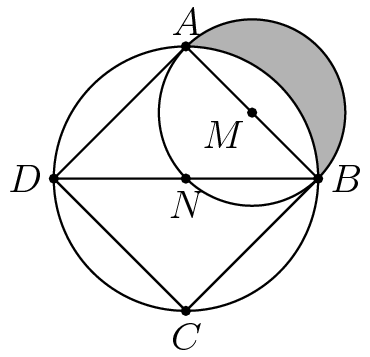
\includegraphics[scale=0.4]{20829b5b2d00796ffd69be6a0a67bde0b0a29dda.png}
    \end{center} 
    
\end{frame}

\refstepcounter{problem}
\begin{frame}[t, fragile]{Problem \thesection.\theproblem}
    \begin{block}{}[Mathcounts]
    %  Concept: Geometry • Difficulty: 5 • Answer: 20 sq units • Solution Available: Yes (Hide) • Report an error with this problem.

 A square and isosceles triangle of equal height are side-by-side, as shown, with both bases on the $x$-axis. The lower right vertex of the square and the lower left vertex of the triangle are at $(10, 0)$. The side of the square and the base of the triangle on the $x$-axis each equal $10$ units. A segment is drawn from the top left vertex of the square to the farthest vertex of the triangle, as shown. What is the area of the shaded region?
    
    \end{block}
    \begin{center}
        \begin{asy}
           /* note: original diagram not to scale, equilateral triangle same height as rectangle */
           import graph; size(140); real lsf=0.5; pen dps=linewidth(0.85)+fontsize(10); defaultpen(dps); pen ds=black; real xmin=-2.2,xmax=23.1,ymin=-2.2,ymax=12.87;
           
           pen zzttqq=dps;
           draw((0,0)--(10,0)--(10,10)--(0,10)--cycle,zzttqq); draw((10,0)--(20,0)--(15,10)--cycle,zzttqq);
           
           Label laxis; laxis.p=fontsize(10); string blank(real x){return "";}
           
           xaxis("$x$",xmin,xmax,defaultpen+black,Arrows(4),above=true); yaxis("$y$",ymin,ymax,defaultpen+black,Arrows(4),above=true); draw((0,0)--(10,0),zzttqq); draw((10,0)--(10,10),zzttqq); draw((10,10)--(0,10),zzttqq); draw((0,10)--(0,0),zzttqq); draw((10,0)--(20,0),zzttqq); draw((0,10)--(20,0)); filldraw((10,0)--(20,0)--intersectionpoints((0,10)--(20,0),(15,10)--(10,0))[0]--cycle,gray(0.7));
           dot((10,0),ds); label("$(10,\,0)$",(10,0),S);
           clip((xmin,ymin)--(xmin,ymax)--(xmax,ymax)--(xmax,ymin)--cycle);
            
        \end{asy}
    \end{center}
   
   \end{frame}
\refstepcounter{problem}
\begin{frame}[t, fragile]{Problem \thesection.\theproblem}
    \begin{block}{}[BmMT 2017]
Take a square $ ABCD $ of side length 1, and let $ P $ be the midpoint of $ AB $. Fold the square so
that point $ D $ touches $ P $, and let the intersection of the bottom edge $ DC $ with the right edge be $ Q $. If $ BQ $ can be expressed as a common fraction $ \frac{a}{b} $, what is $ a + b? $
    \end{block}
    \begin{center}
        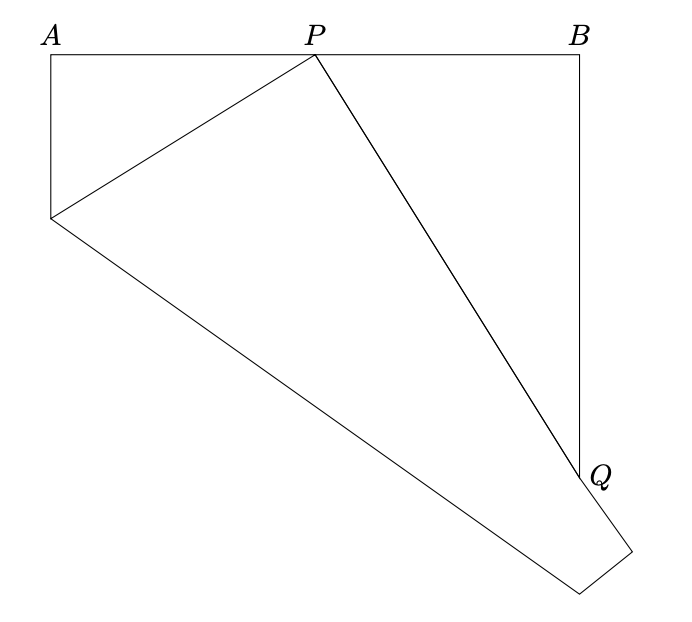
\includegraphics[scale=0.5]{bmmt_17_16}
    \end{center}
    
    \end{frame}



\refstepcounter{problem}
\begin{frame}[t, fragile]{Problem \thesection.\theproblem}
    \begin{block}{}[Mathcounts 2014-15 Handbook, \#248]
    In the figure, $\overarc{CBD}$ is a semicircle with center $O$ and diameter $CD$. If is a semicircle with center $O$ and diameter $CD$. If $AB = OD$ and the measure of angle $EOD$ is 60 degrees, what is the measure of angle $A$?
    \end{block}
    \begin{center}
        \begin{asy}
  import cse5;
  unitsize(0.5cm);
  pair A, A1, B, C, D, E, O;
path semi;

O = (0, 0);
D = (3, 0);
C = (-3, 0);

semi = arc(O, 3, 0, 180);
draw(semi);
draw(C--D);
E = rotate(60,O)*D;
draw(O--E);
A1 = rotate(200,E)*(E.x+1, E.y);
A = extension(E, A1, D, C);
B = intersectionpoint(A1--A, semi);
draw (E--A);
draw (A--C);
//draw (O--B, dashed);

label("$A$", A, S);
label("$B$", B, NW);
label("$C$", C, S);
label("$D$", D, S);
label("$E$", E, NE);
label("$O$", O, S);
/*
MA("\alpha", C, A, B, 1);
MA("\alpha", B, O, C, 1);
MA("\beta", O, B, E, 1);
MA("\beta", B, E, O, 1);
MA("60^\circ", D, O, E, 1);
*/
\end{asy}

    \end{center}
     
\end{frame}

\refstepcounter{problem}
\begin{frame}[t, fragile]{Problem \thesection.\theproblem}
    \begin{block}{}[Mathcounts 2017 State, Sprint \#22]
     Chloe finds a coin, as shown, wedged tightly into the corner of her drawer behind a rectangular box with a 2.5-inch edge. One corner of the box is 1.5 inches from the corner of the drawer and the other corner of the box is 2 inches from the corner of the drawer. What is the diameter of the coin in inches?

    \end{block}

    \begin{center}
        \begin{asy}
              import cse5;
              unitsize(0.75cm);
              import olympiad;
              pair A,B,C,O,I, B1, C1;
              A=(0,0); B=(1.5,0); C=(0,2.5);
              O=circumcenter(A,B,C);
              I=incenter(A,B,C);
              //draw(A--B--C--cycle);
              draw(A--(3,0));
              draw(A--(0,3));
              draw(B--C);
              //dot(I);
              draw(incircle(A,B,C));
            
              B1 = rotate(-90,B)*((C+B)/2);
              C1 = rotate(90, C)*((C+B)/2);
              filldraw (B--B1--C1--C--cycle, lightgrey);
        \end{asy}
    \end{center}
    
\end{frame}

%-------------------------
\section{Challenge Practice Problems}

\refstepcounter{problem}
\begin{frame}[t, fragile]{Problem \thesection.\theproblem}
    \begin{block}{}[Mathcounts National 2017, Sprint \#13]
     In right triangle $ABC$ with right angle at vertex $C$, a semicircle is constructed,
    as shown, with center $P$ on leg $AC$, so that the semicircle is tangent to leg $BC$
    at $C$, tangent to the hypotenuse $AB$, and intersects leg $AC$ at $Q$ between
    $A$ and $C.$ The ratio of $AQ$ to $QC$ is $2:3.$ If $BC = 12,$ then what is the
    value of $AC?$ Express your answer in simplest radical form.    
    \end{block}
    \begin{center}
        \begin{asy}
            import olympiad;
            unitsize(0.25cm);
            pair A, B, C, O, T;
            real r = 24/sqrt(10);
            C = (0, 0);
            B = (0, 12);
            A = (-8*sqrt(10), 0);
            O = (-r, 0);
            T = foot(O, A, B);
            
            draw(A--B--C--cycle);
            draw(arc(O, r, 0, 180));
    
            dot(O);
            //dot(T);
            label("$A$", A, SW);
            label("$C$", C, SE);
            label("$B$", B, NE);
            label("$P$", O, S);
            label("$Q$", O*2, S);
            
        \end{asy}    
        \end{center}
        
    \end{frame}

% Manoj - This could be intermediate as well?
\refstepcounter{problem}
\begin{frame}[t, fragile]{Problem \thesection.\theproblem}
    \begin{block}{}[Mathcounts 2015 National, Sprint \#27]
     An equilateral triangle shares a side with a square, and a circle is inscribed between them, as shown. If the radius of the circle is $9 - 3\sqrt{3}$ , what is the side length of the square?

    \end{block}
    \begin{center}
        \begin{asy}
             unitsize (1cm);
             real r = 1, s = 3 + sqrt(3);
             pair O, A, B, C, D, E;
             O = (0, 0);
             A = (r, r);
             B = (r, r-s);
             C = (r-s, r-s);
             D = (r-s, r);
             E = rotate (-60, B)*C;
             
             draw(A--B--C--D--cycle);
             draw (B--E--C);
             draw(circle(O, r));
        \end{asy}
    \end{center}
    
\end{frame}

% Manoj - This could be intermediate as well?
\refstepcounter{problem}
\begin{frame}[t, fragile]{Problem \thesection.\theproblem}
    \begin{block}{}[Mathcounts 2015 National, Sprint \#25]
     Right triangle $ABC$ has side lengths $AB = 4$ cm, $BC = 3$ cm
and $AC = 5$ cm. $A$ also is a vertex of a square, and $B$ and $C$ lie
on two sides of the square as shown. What is the area of the
square? Express your answer as a common fraction.

     
    \end{block}
    \begin{center}
        \begin{asy}
            import olympiad;
             unitsize (3cm);
             pair A, B, C, D, E, F;
           
             A = (1, 0);
             B = (0, 1/4);
             C = (3/16, 1);
             D = (1, 1);
             E = (0, 1);
             F = (0, 0);
             
             draw (A--B--C--cycle);
             draw (A--D--E--F--cycle);
             draw(rightanglemark(A, B, C, 2), black);
           
             label("$A$", A, SE);
             label("$B$", B, W);
             label ("$C$", C, N);
             
        \end{asy}
    \end{center}
\end{frame}



\refstepcounter{problem}
\begin{frame}[t, fragile]{Problem \thesection.\theproblem}
    \begin{block}{}[Mathcounts 2014 National Target \#8]
     A circle passes through two diagonally opposite vertices of a 3-inch by 4-inch rectangle. What is the least possible distance between the center of the circle and a vertex of the rectangle? Express your answer as a common fraction. 
	
    \end{block}
\end{frame}

\end{document}
